\documentclass[10pt,conference,compsocconf]{IEEEtran}

\usepackage{hyperref}
\usepackage{graphicx}	% For figure environment
\usepackage{caption}


\begin{document}
\title{The Higgs boson Machine Learning Challenge}

\author{
  Emanuele Nevali, Matteo Suez, Leonardo Bruno Trentini\\
  \textit{Machine Learning and Optimization Laboratory, EPFL, Switzerland}
}

\maketitle

\begin{abstract}
In this project, carried out as part of the 2022 Machine Learning course at EPFL, we applied machine learning techniques to actual CERN particle accelerator data to recreate the process of
“discovering” the Higgs particle.\\
\end{abstract}

\section{Introduction}
Rarely, collisions between protons at high speed can produce a Higgs boson, an elementary and unstable particle in the Standard Model of particle physics theory\cite{faq}. Since this boson decays rapidly into other particles, it is not possible to observe it directly, but rather measure its “decay signature”, or the products that result from its decay process. The aim of this project is to estimate the likelihood that a given event’s signature was the result of a Higgs boson (signal) or some other process/particle (background).\\
After analysis and preprocessing of the dataset, we introduce the model built with the 6 demanded algorithms and we explain how we managed to choose the best hyperparameters. In conclusion, we present our results.

\section{Data analysis and preprocessing}

\subsection{Exploratory data analysis}
Our dataset contains 250000 points for training and 568238
for testing with their corresponding binary label (“s” for “signal” and “b” for “background”, which have to be predicted for the test set values). All of these points are characterized by 30 different features. \\
\vspace{-0.8cm}\\

\subsection{Categorization}
First of all, we notice that there is only one categorical feature, i.e. \textit{Pri jet num}: it shows the number of jets (see \cite{higgs} for a physical explanation), and it is an integer that ranges from 0 to 3. \\
We noticed that some features are meaningless for some values of jets, therefore we have split the dataset into 4 subclasses, each one characterized by a different \textit{Pri jet num}.\\
\vspace{-0.8cm}\\

\subsection{Missing Values}
Thanks to the documentation, we noticed that each “-999” value
in the dataset consists in a missing value: we decided to replace all of them with the median of the feature. In particular, we chose to use the median instead of the mean because of its nature of robust estimator to outliers.\\
\begin{figure}[h]
    \centering
    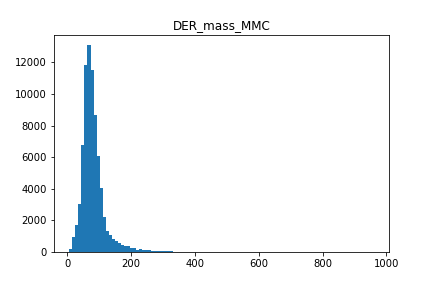
\includegraphics[width=0.237\textwidth]{report/HeavyTail_before_log.png}
    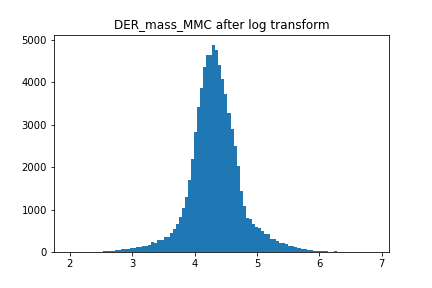
\includegraphics[width=0.237\textwidth]{report/HeavyTail_after_log.png}
    \caption{Logarithmic transformation for the 1st feature}
    \label{fig:lambdas}
\end{figure}
Furthermore, for subclasses marked by \textit{Pri jet num} $0$ and $1$ we decided not to consider columns with too many missing values, in order to avoid singular matrices.\\
\vspace{-0.8cm}\\

\subsection{Absolute transform of Symmetrical Features}
For features whose distribution is symmetric around 0 and for which the proportion of categories is not too even, we replaced them with their absolute value.\\
This operation increases the gap between the categories, and makes them more detectable by the model. \\
\vspace{-0.8cm}\\

\subsection{Outliers threshold}
After a search for outliers in the data, we set $\alpha = 0.05$ and decided to edge the extreme values of each feature to the $\alpha$-quantile (for the lower tail) and to the $(1-\alpha)$-quantile (for the upper tail).\\
\vspace{-0.8cm}\\

\subsection{Angles}
We noticed that some of the features represents measurements of angles. For this reason, in order to adapt our model to the periodicity of this type of data, we tried to replace these columns with sine and cosine transformations. However, only the latter appeared to be effective, and it was the only one kept in the final model.\\
\vspace{-0.8cm}\\

%\subsection{Correlated features}
%We observed that the empirical distribution of some of the features was too similar, index of an high correlation between them. By not considering these features, we slightly improved our performance.\\
%\vspace{-0.8cm}\\

\subsection{Heavy-tailed features}
Noticing that many of the features were heavy-tailed, we computed for these a logarithmic transformation: $x_{k}^{*} = log(1+x_k)$ (where $k$ is the feature column). These transformation  helps in reducing or removing the skewness of our original data.\\
\vspace{-0.8cm}\\

\subsection{Standardization}
In order to ensure a better functioning of our algorithms, we decided to standardize the data by subtracting from each feature its mean and dividing by its standard deviation: 

\begin{center}
\label{fig:accuracytab}
\scalebox{0.7}{\begin{tabular}{|c|c c c c|c|}
\hline
Method & Subset 1 & Subset 2 & Subset 3 & Subset 4 & Total\\
\hline
Gradient Descent & 70.7\% & 65.4\% & 67.9\% & 68.3\% & 68.3\%\\
Stochastic Gradient Descent & 69.8\% & 66.6\% & 67.5\% & 68.5\% & 68.2\%\\
Least squares & 84.6\% & 81.1\% & 84.4\% & 84.1\% & 83.5\%\\
Ridge regression & 84.7\% & 81.3\% & 84.7\% & 84.5\% & 83.6\%\\
Logistic regression & 77.1\% & 68.6\% & 67.1\% & 69.8\% & 71.8\%\\
Regularized logistic & 76.6\% & 69.1\% & 66.7\% & 69.8\% & 71.6\%\\
\hline
Variance & \multicolumn{5}{|c|}{$\pm 10^{-3}$}\\
\hline
\end{tabular}}\\
\captionof{table}{Accuracies for each method and subset. The average was weighted on the number of points for each subset}
\end{center}
\vspace{0.1cm}\\

$Z=\frac{X-\mu}{\sigma}$. The same process was applied both to the train set and to the test set, using on the latter $\mu$ and $\sigma$ of the former.\\
\vspace{-0.8cm}\\

\subsection{Polynomial Expansion}
We managed to improve our predictions by expanding the features In particular, we augmented features by implementing a polynomial expansion for each column of the form $\phi:[X]\rightarrow [X,X^2,...,X^D]$.\\
The polynomial degree $D$ is one of the hyper-parameters of our model: we found its optimal value by performing a 4-fold cross validation on each subset.\\
In addition, we decided to add for each couple of features a new feature with their product, and to compute the square root and the cubic root of each feature. This last operations improved significantly the accuracy of the model.\\
\vspace{-0.6cm}\\

\section{Methods}
After the pre-processing on the dataset, we managed to find a model for our problem by implementing six different methods:
\begin{itemize}
    \item \textbf{Gradient Descent}
    \item \textbf{Stochastic Gradient Descent}
    \item \textbf{Least squares} using normal equations
    \item \textbf{Ridge regression} using normal equations
    \item \textbf{Logistic regression} using gradient descent or stochastic gradient descent ($y \in {0,1}$)
    \item \textbf{Regularized logistic regression} using gradient descent or stochastic gradient descent ($y \in {0,1}$, with regularization term $ \lambda  \| \omega \|^2$)
\end{itemize}
All functions return: (w, loss), which is the last weight vector of the
method, and the corresponding loss value (or cost function).\\
\vspace{0.05cm}\\
Optimal parameters $\lambda$ (regularization to reduce overfitting), $\gamma$ (step size for gradient and stochastic gradient descent) and $D$ (degrees for polynomial expansion) were chosen through a 4-fold cross validation for each subset.
\begin{figure}[h]
    \centering
    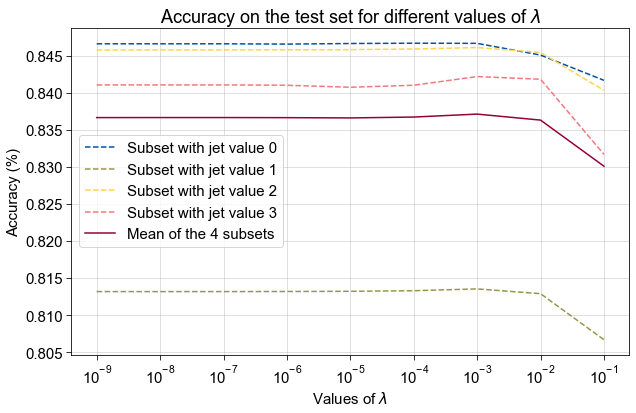
\includegraphics[width=0.4\textwidth]{report/lambdas2.png} \\
    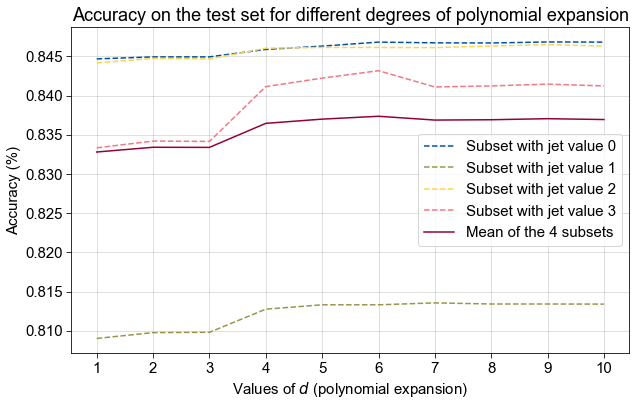
\includegraphics[width=0.4\textwidth]{report/degrees2.png}
    \caption{Accuracy for different values of $\lambda$ and $D$}
    \label{fig:lambdas}
\end{figure}\\


\section{Results}
Due to the fact that we were facing a binary classification problem, we first focused on the Regularized Logistic Regression. However, in the meanwhile we also carried out multiple tests with Least Squares and Ridge Regression, and remarkably the latter turned out to be the most effective method.\\
For this reason, we focused on calibrating Ridge Regression hyperparameters. We did it by using grid-search method and 4-fold cross-validation, looking for the best compromise between underfitting and overfitting. We adjusted the hyperparameters for each of the four subclasses.\\
At the end, we obtained a model that achieved an accuracy of 0.837 on AIcrowd platform.


\section{Conclusions}
The best performance on the Higgs boson
challenge, with an accuracy on the test set of 0.837, was obtained with a Ridge Regression.\\
It is important to underline that data analysis, data cleaning and feature preprocessing played a key role in this task, enabling us to achieve massive improvements in model's accuracy.\\



\bibliographystyle{IEEEtran}
\bibliography{literature}

\end{document}